% Original vector reconstruction of source Fig.75.2, PDF305.
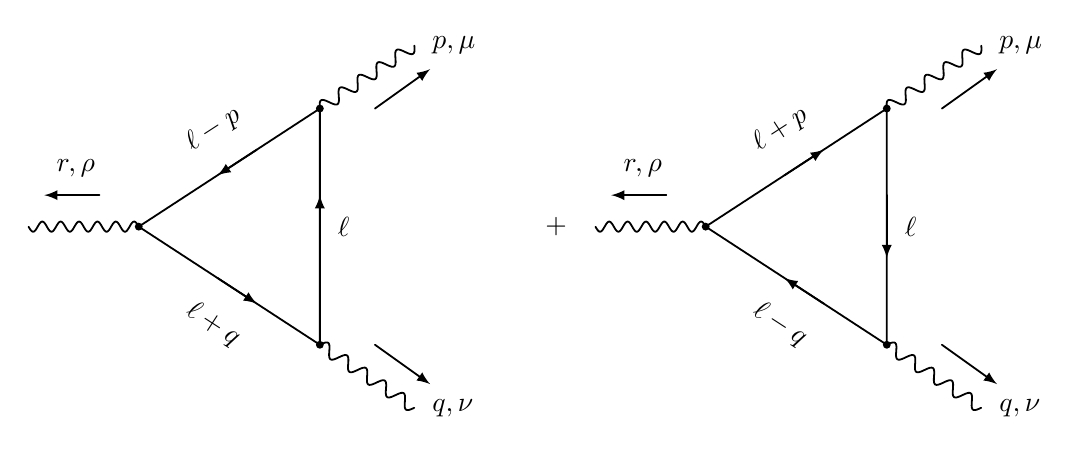
\begin{tikzpicture}[x=1mm,y=1mm,line width=.65pt,>=latex,
 line cap=round,line join=round,font=\fontsize{10}{12}\selectfont]
\foreach \offset/\reverse in {0/0,72/1}{
\begin{scope}[xshift=\offset mm]
\coordinate (R) at (10,0);
\coordinate (M) at (33,15);
\coordinate (N) at (33,-15);
\draw (R)--(M)--(N)--cycle;
\ifnum\reverse=0
 \draw[->] (25,9.78)--(20,6.52);
 \draw[->] (20,-6.52)--(25,-9.78);
 \draw[->] (33,-4)--(33,4);
 \node[above,rotate=33] at (21,10) {$\ell-p$};
 \node[below,rotate=-33] at (21,-10) {$\ell+q$};
\else
 \draw[->] (20,6.52)--(25,9.78);
 \draw[->] (25,-9.78)--(20,-6.52);
 \draw[->] (33,4)--(33,-4);
 \node[above,rotate=33] at (21,10) {$\ell+p$};
 \node[below,rotate=-33] at (21,-10) {$\ell-q$};
\fi
\node[right] at (34,0) {$\ell$};
\draw[domain=0:1,samples=101,smooth,variable=\u]
 plot ({10-14*\u},{.65*sin(2160*\u)});
\draw[domain=0:1,samples=101,smooth,variable=\u]
 plot ({33+12*\u-.45*sin(1800*\u)},{15+8*\u+.65*sin(1800*\u)});
\draw[domain=0:1,samples=101,smooth,variable=\u]
 plot ({33+12*\u+.45*sin(1800*\u)},{-15-8*\u+.65*sin(1800*\u)});
\draw[->] (5,4)--(-2,4);
\node[above] at (2,5) {$r,\rho$};
\draw[->] (40,15)--(47,20);
\draw[->] (40,-15)--(47,-20);
\node[right] at (46,23) {$p,\mu$};
\node[right] at (46,-23) {$q,\nu$};
\foreach \a in {R,M,N}{\fill (\a) circle[radius=.5mm];}
\end{scope}
}
\node at (63,0) {$+$};
\end{tikzpicture}
